\documentclass[aspectratio=169, 11pt]{beamer}

% Minimal theme — no colored bars, no ornaments
\usetheme{default}
\usecolortheme{default}

% Strip all beamer chrome
\setbeamertemplate{navigation symbols}{}
\setbeamertemplate{headline}{}
\setbeamertemplate{footline}{
  \hfill{\color{mpGray}\footnotesize\insertframenumber/\inserttotalframenumber}\hspace{0.6cm}\vspace{0.4cm}
}

% Colors — white base, teal accent only
\definecolor{mpTeal}{HTML}{0D9373}
\definecolor{mpDark}{HTML}{1A1A1A}
\definecolor{mpGray}{HTML}{888888}
\definecolor{mpLightGray}{HTML}{E5E5E5}
\definecolor{mpRed}{HTML}{B33A3A}

% Everything on white
\setbeamercolor{background canvas}{bg=white}
\setbeamercolor{normal text}{fg=mpDark}
\setbeamercolor{frametitle}{fg=mpDark, bg=white}
\setbeamercolor{title}{fg=mpDark, bg=white}
\setbeamercolor{subtitle}{fg=mpGray}
\setbeamercolor{author}{fg=mpGray}
\setbeamercolor{date}{fg=mpGray}
\setbeamercolor{structure}{fg=mpTeal}
\setbeamercolor{item}{fg=mpTeal}
\setbeamercolor{block title}{fg=mpDark, bg=mpLightGray}
\setbeamercolor{block body}{fg=mpDark, bg=white}
\setbeamercolor{block title alerted}{fg=mpRed, bg=white}

% Clean fonts
\setbeamerfont{title}{size=\LARGE, series=\bfseries}
\setbeamerfont{subtitle}{size=\normalsize, series=\mdseries}
\setbeamerfont{frametitle}{size=\large, series=\bfseries}
\setbeamerfont{block title}{size=\normalsize, series=\bfseries}

% Thin line under frame title
\setbeamertemplate{frametitle}{
  \vspace{0.4cm}
  \insertframetitle
  \vspace{0.15cm}
  {\color{mpLightGray}\hrule height 0.5pt}
  \vspace{0.2cm}
}

% Simple title page
\setbeamertemplate{title page}{
  \vspace{2cm}
  {\usebeamerfont{title}\usebeamercolor[fg]{title}\inserttitle}\\[0.3cm]
  {\usebeamerfont{subtitle}\usebeamercolor[fg]{subtitle}\insertsubtitle}\\[1cm]
  {\usebeamercolor[fg]{author}\insertauthor}\\[0.2cm]
  {\usebeamercolor[fg]{date}\insertdate}
}

\usepackage{booktabs}
\usepackage{graphicx}
\usepackage{tikz}
\usetikzlibrary{arrows.meta, positioning, shapes.geometric}

\title{MomoParse}
\subtitle{User-Owned Financial Intelligence from Mobile Money SMS}
\author{Alex Marfo}
\date{March 2026}

\begin{document}

% ============================================================
% TITLE
% ============================================================
\begin{frame}
\titlepage
\end{frame}

% ============================================================
% OUTLINE
% ============================================================
\begin{frame}{Outline}
\tableofcontents
\end{frame}

% ============================================================
\section{The Market}
% ============================================================

\begin{frame}{Ghana's Mobile Money Market}
\begin{columns}[T]
\begin{column}{0.5\textwidth}
\begin{block}{Scale (2024)}
\begin{itemize}
  \item \textbf{74.1M} registered wallets
  \item \textbf{8.1B} transactions/year
  \item \textbf{GH\textcent 3.01T} total value
  \item \textbf{60\%} of Ghanaians 15+ have an account
  \item \textbf{GH\textcent 372} avg transaction
\end{itemize}
\end{block}
\end{column}
\begin{column}{0.5\textwidth}
\begin{block}{Growth}
\begin{itemize}
  \item 2025 pace: \textbf{GH\textcent 3.6T} (Jan--Oct)
  \item Transaction volume: \textbf{+18.9\%} YoY
  \item Transaction value: \textbf{+56.8\%} YoY
  \item GhIPSS Instant Pay: \textbf{+233\%} YoY
  \item Market projected: \textbf{USD 934B by 2033}
\end{itemize}
\end{block}
\end{column}
\end{columns}

\vspace{0.5cm}
\centering
\textcolor{mpTeal}{\textbf{Every transaction generates an SMS confirmation.\\8.1 billion unstructured text records per year.}}
\end{frame}

% ============================================================
\begin{frame}{Regulatory Caps --- Bank of Ghana KYC Tiers}
\centering
\begin{tabular}{l c c c}
\toprule
& \textbf{Minimum} & \textbf{Medium} & \textbf{Enhanced} \\
\midrule
\textbf{KYC Required} & Ghana Card & + Next of kin & + Proof of address \\
\textbf{Daily Limit} & GH\textcent 3,000 & GH\textcent 15,000 & GH\textcent 25,000 \\
\textbf{Monthly Limit} & GH\textcent 10,000 & Unlimited & Unlimited \\
\textbf{Max Balance} & GH\textcent 5,000 & GH\textcent 40,000 & GH\textcent 75,000 \\
\bottomrule
\end{tabular}

\vspace{0.6cm}
Most Ghanaians sit at \textbf{Minimum KYC} --- the least financial visibility,\\the most to gain from a tool like MomoParse.
\end{frame}

% ============================================================
\section{The Problem}
% ============================================================

\begin{frame}{The Data Asymmetry}
\small
\begin{columns}[T]
\begin{column}{0.48\textwidth}
\begin{block}{What telcos know about you}
\begin{itemize}\setlength{\itemsep}{2pt}
  \item Transaction history, frequency, volume
  \item Recharge patterns, top-up consistency
  \item Call data records, contact diversity
  \item Location data, device behavior, tenure
\end{itemize}
\end{block}
\end{column}
\begin{column}{0.48\textwidth}
\begin{block}{What they do with it}
\begin{itemize}\setlength{\itemsep}{2pt}
  \item \textbf{Credit scoring} --- TransUnion partnership
  \item \textbf{Loan limits} --- Qwikloan, txn-based
  \item \textbf{Airtime advance} --- loyalty-based ceiling
  \item \textbf{Pricing} --- Just4U personalized bundles
\end{itemize}
\end{block}
\end{column}
\end{columns}

\vspace{0.6cm}
\centering
\textcolor{mpRed}{\textbf{The user never sees this score. Can't export it. Can't challenge it.}}
\end{frame}

% ============================================================
\section{The Infrastructure}
% ============================================================

\begin{frame}{How a MoMo Transaction Works}
\centering
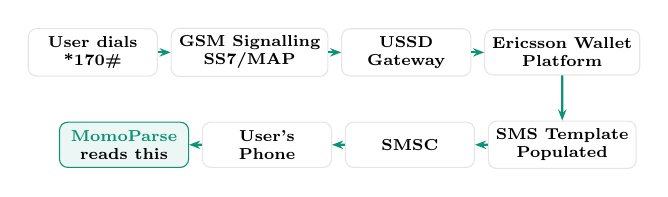
\begin{tikzpicture}[scale=0.82, transform shape,
  node distance=0.5cm and 0.2cm,
  every node/.style={font=\scriptsize, align=center},
  box/.style={rectangle, draw=mpLightGray, fill=white, rounded corners=3pt,
              minimum height=0.7cm, minimum width=2cm, font=\scriptsize\bfseries},
  arr/.style={-{Stealth[length=4pt]}, thick, color=mpTeal}
]
  \node[box] (ussd)  {User dials\\*170\#};
  \node[box, right=of ussd]  (gsm)   {GSM Signalling\\SS7/MAP};
  \node[box, right=of gsm]   (gw)    {USSD\\Gateway};
  \node[box, right=of gw]    (ewp)   {Ericsson Wallet\\Platform};
  \node[box, below=0.7cm of ewp]   (sms)   {SMS Template\\Populated};
  \node[box, left=of sms]    (smsc)  {SMSC};
  \node[box, left=of smsc]   (phone) {User's\\Phone};
  \node[box, left=of phone, fill=mpTeal!8, draw=mpTeal]  (mp)    {\textcolor{mpTeal}{MomoParse}\\reads this};

  \draw[arr] (ussd) -- (gsm);
  \draw[arr] (gsm)  -- (gw);
  \draw[arr] (gw)   -- (ewp);
  \draw[arr] (ewp)  -- (sms);
  \draw[arr] (sms)  -- (smsc);
  \draw[arr] (smsc) -- (phone);
  \draw[arr] (phone) -- (mp);
\end{tikzpicture}

\vspace{0.3cm}
\small
\begin{itemize}\setlength{\itemsep}{2pt}
  \item Ericsson Wallet Platform: \textbf{400M+ wallets}, \textbf{2.8B txns/month} globally
  \item SMS confirmations are \textbf{template-generated} --- consistent, parseable, reliable
  \item GhIPSS handles cross-network interop (MTN $\leftrightarrow$ Telecel $\leftrightarrow$ Banks)
\end{itemize}
\end{frame}

% ============================================================
\section{The Gap}
% ============================================================

\begin{frame}{Competitive Landscape}
\centering
\small
\begin{tabular}{l l l l}
\toprule
\textbf{Player} & \textbf{Approach} & \textbf{Access} & \textbf{Gap} \\
\midrule
MTN / Telecel    & Internal scoring    & Proprietary    & Users can't see their score \\
Pngme (\$18M)    & Phone SDK           & Enterprise     & Invasive, opaque, closed \\
Mono / Stitch    & Bank APIs           & Developer      & Banks, not mobile money \\
Okra             & Bank APIs           & ---            & Collapsed May 2025 \\
PawaPay / Tola   & Payment aggregation & Developer      & Move money, don't analyze it \\
MTN MoMo API     & 30 payment APIs     & Developer      & Forward-looking, not history \\
\midrule
\textcolor{mpTeal}{\textbf{MomoParse}} & \textcolor{mpTeal}{\textbf{SMS $\rightarrow$ API}} & \textcolor{mpTeal}{\textbf{Open}} & \textcolor{mpTeal}{\textbf{This space is empty}} \\
\bottomrule
\end{tabular}
\end{frame}

% ============================================================

\begin{frame}{Market Positioning}
\centering
\vspace{0.3cm}
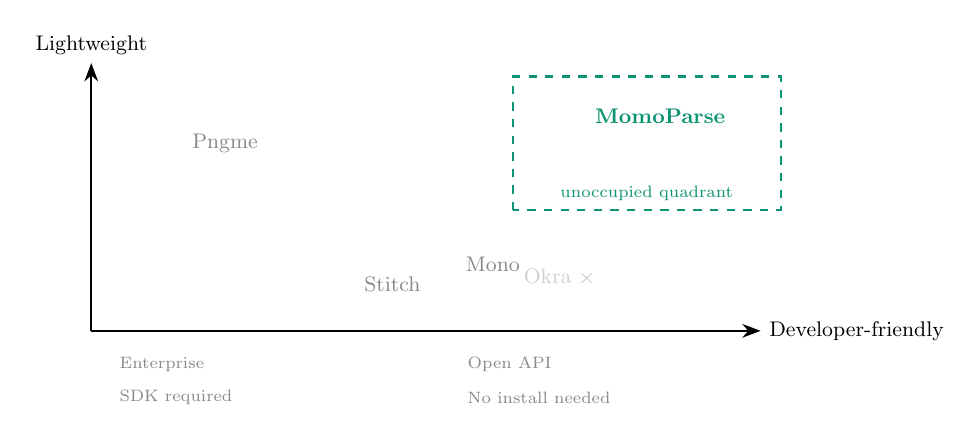
\begin{tikzpicture}[scale=0.85, transform shape]
  \draw[-{Stealth}, thick] (0,0) -- (10,0) node[right, font=\small] {Developer-friendly};
  \draw[-{Stealth}, thick] (0,0) -- (0,4) node[above, font=\small] {Lightweight};

  \node[font=\small, text=mpGray] at (2, 2.8) {Pngme};
  \node[font=\small, text=mpGray] at (6, 1) {Mono};
  \node[font=\small, text=mpGray] at (4.5, 0.7) {Stitch};
  \node[font=\small, text=mpGray, opacity=0.4] at (7, 0.8) {Okra \texttimes};
  \node[font=\small\bfseries, text=mpTeal] at (8.5, 3.2) {MomoParse};

  \draw[mpTeal, thick, dashed] (6.3, 1.8) rectangle (10.3, 3.8);
  \node[font=\scriptsize, text=mpTeal] at (8.3, 2.05) {unoccupied quadrant};

  \node[font=\scriptsize, text=mpGray, anchor=west] at (0.3, -0.5) {Enterprise};
  \node[font=\scriptsize, text=mpGray, anchor=west] at (0.3, -1) {SDK required};
  \node[font=\scriptsize, text=mpGray, anchor=west] at (5.5, -0.5) {Open API};
  \node[font=\scriptsize, text=mpGray, anchor=west] at (5.5, -1) {No install needed};
\end{tikzpicture}
\end{frame}

% ============================================================
\section{The Solution}
% ============================================================

\begin{frame}{MomoParse --- Inverting the Power Dynamic}
\begin{columns}[T]
\begin{column}{0.48\textwidth}
\begin{block}{The Telco Way (closed)}
\begin{enumerate}
  \item Internal transaction database
  \item Proprietary scoring algorithm
  \item Locked credit score
  \item Telco decides your loan limit
  \item \textcolor{mpRed}{User never sees why}
\end{enumerate}
\end{block}
\end{column}
\begin{column}{0.48\textwidth}
\begin{block}{The MomoParse Way (open)}
\begin{enumerate}
  \item User-owned SMS confirmations
  \item Open parsing + ML categorization
  \item Transparent financial indexes
  \item User owns their profile
  \item \textcolor{mpTeal}{Portable, challengeable}
\end{enumerate}
\end{block}
\end{column}
\end{columns}

\vspace{0.5cm}
\centering
\textbf{Same data origin. Same signals. Different owner.}
\end{frame}

% ============================================================
\section{Signal Mapping}
% ============================================================

\begin{frame}{Telco Signals vs.\ MomoParse Signals}
\centering
\small
\begin{tabular}{l l l}
\toprule
\textbf{Telco Signal (Internal)} & \textbf{MomoParse (From SMS)} & \textbf{Meaning} \\
\midrule
Top-up frequency       & Income txn frequency       & Income stability \\
Transaction volume     & Total inflows/outflows     & Cash flow capacity \\
Recharge consistency   & Spending regularity        & Financial discipline \\
CDR contact diversity  & Counterparty diversity     & Economic breadth \\
Loan repayment history & Recurring payment patterns & Reliability \\
ARPU                   & Avg transaction size       & Economic tier \\
\midrule
Location data          & \textcolor{mpRed}{\textit{Not available}}  & --- \\
Battery/device habits  & \textcolor{mpRed}{\textit{Not available}}  & --- \\
\bottomrule
\end{tabular}

\vspace{0.5cm}
MomoParse approximates \textbf{6 of 8} key telco credit scoring signals\\using \textbf{only user-owned SMS data}. No proprietary access needed.

\vspace{0.2cm}
\textcolor{mpGray}{\footnotesize The 2 missing signals require invasive device access --- the tradeoff is transparency and user ownership.}
\end{frame}

% ============================================================
\section{Financial Indexes}
% ============================================================

\begin{frame}{Scoring Methodology --- Grounded in Finance}
\centering
\small
\begin{tabular}{l l l}
\toprule
\textbf{Index} & \textbf{Formula} & \textbf{Maps To} \\
\midrule
Savings Rate & $\dfrac{\text{Income} - \text{Expenses}}{\text{Income}}$ & Personal finance standard \\[8pt]
Transaction Velocity & $\dfrac{\text{Transactions}}{\text{Period}}$ & CDR frequency (telco) \\[8pt]
Income Stability & $\sigma(\text{income across periods})$ & Top-up consistency \\[8pt]
Counterparty Concentration & Herfindahl index of partners & Contact diversity \\[8pt]
Expense Volatility & $\sigma(\text{spending month-to-month})$ & Recharge pattern scoring \\
\bottomrule
\end{tabular}

\vspace{0.5cm}
Each formula is \textbf{citable} in finance literature,\\\textbf{maps to a known telco scoring factor}, and is \textbf{transparent to the user}.
\end{frame}

% ============================================================
\section{Architecture}
% ============================================================

\begin{frame}{Technical Architecture}
\centering
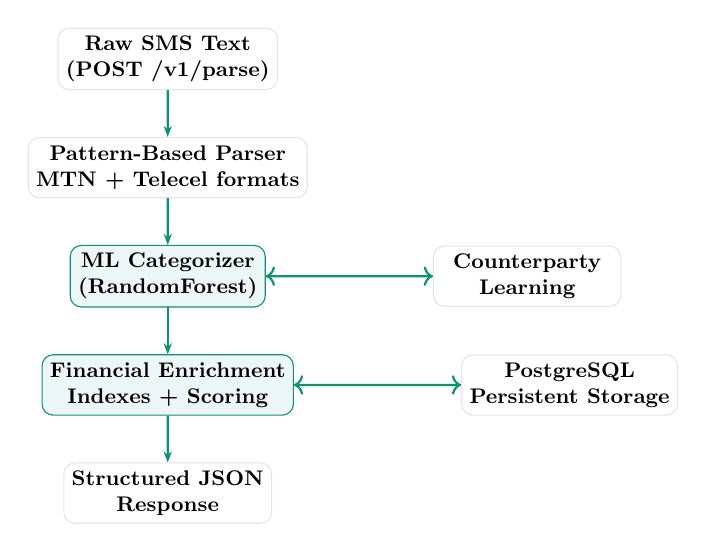
\begin{tikzpicture}[scale=0.85, transform shape,
  node distance=0.7cm,
  every node/.style={font=\small, align=center},
  box/.style={rectangle, draw=mpLightGray, fill=white, rounded corners=4pt,
              minimum height=0.9cm, minimum width=2.8cm, font=\small\bfseries},
  mlbox/.style={box, fill=mpTeal!8, draw=mpTeal},
  arr/.style={-{Stealth[length=4pt]}, thick, color=mpTeal}
]
  \node[box] (input) {Raw SMS Text\\(POST /v1/parse)};
  \node[box, below=of input] (parser) {Pattern-Based Parser\\MTN + Telecel formats};
  \node[mlbox, below=of parser] (ml) {ML Categorizer\\(RandomForest)};
  \node[mlbox, below=of ml] (enrich) {Financial Enrichment\\Indexes + Scoring};
  \node[box, below=of enrich] (output) {Structured JSON\\Response};

  \node[box, right=2.5cm of ml] (cp) {Counterparty\\Learning};
  \node[box, right=2.5cm of enrich] (db) {PostgreSQL\\Persistent Storage};

  \draw[arr] (input) -- (parser);
  \draw[arr] (parser) -- (ml);
  \draw[arr] (ml) -- (enrich);
  \draw[arr] (enrich) -- (output);
  \draw[arr, <->] (ml) -- (cp);
  \draw[arr, <->] (enrich) -- (db);
\end{tikzpicture}
\end{frame}

% ============================================================
\section{The Thesis}
% ============================================================

\begin{frame}{The Thesis}
\centering
\vspace{1cm}

\begin{beamercolorbox}[sep=1em, center, rounded=true, shadow=true]{block title}
\large
``In a market of 74 million wallets and GH\textcent 3 trillion\\in annual transactions, telcos score users with proprietary\\algorithms the user never sees.

\vspace{0.5cm}

MomoParse extracts the same financial signals from\\user-owned SMS data --- transparently, through an open API ---\\giving users and developers access to financial intelligence\\that was previously locked inside telco systems.''
\end{beamercolorbox}

\vspace{1cm}
\textcolor{mpGray}{User-side financial intelligence for mobile money.}
\end{frame}

% ============================================================
\begin{frame}{Thank You}
\centering
\vspace{1.5cm}

{\Large\bfseries MomoParse}

\vspace{0.3cm}
{\textcolor{mpGray}{User-Owned Financial Intelligence from Mobile Money SMS}}

\vspace{1.5cm}

Alex Marfo\\
\textcolor{mpTeal}{github.com/theboylexis/momo-parse-api}

\vspace{1cm}
\textcolor{mpGray}{\footnotesize March 2026}
\end{frame}

\end{document}
